\documentclass[11pt,a4paper]{article}
\usepackage[czech]{babel}
\usepackage[utf8]{inputenc}
\usepackage{times}
\usepackage{url}
\usepackage[textwidth=15.2cm,textheight=23cm]{geometry}
\usepackage{xcolor}

\usepackage{graphicx}

%\usepackage{fancyvrb}
%\DefineVerbatimEnvironment{verbatim}{Verbatim}{}

\usepackage[bf]{caption}

\usepackage[hyperindex,
  plainpages=false,
%  pdftex,
  colorlinks,
  pdfborder={0 0 0},
  pdfpagelabels]{hyperref}

\pdfcompresslevel=9

\newcommand{\myincludegraphics}[4]{
  \begin{figure}[!h]
  \centering
  \includegraphics[#1]{#2}
  \caption{#3.} \label{#4}
  \end{figure}
}

% titulní stránka a obsah
\newcommand{\titlepageandcontents}{
  \begin{titlepage}

\vspace*{1cm}

\begin{figure}
  \centering
  
\includegraphics[height=6cm]{images/fit}
\end{figure}

\vspace*{5mm}

\begin{center}
\begin{Large}
Projekt do předmětu GMU -- Grafické a multimediální procesory
\end{Large}
\end{center}

\vspace*{5mm}

\begin{center}
\begin{Huge}
pr05\\Urychlení metod k-means a mean-shift pomocí 3D akcelerační karty (OpenCL/CUDA) \\
\end{Huge}
\end{center}

\vspace*{1cm}

\begin{center}
\begin{Large}
\today
\end{Large}
\end{center}

\vfill

\begin{flushleft}
\begin{large}
\begin{tabular}{ll}

\bf Řešitelé:\hspace{3mm} & Martin Šimon (\verb_xsimon14@stud.fit.vutbr.cz_) \\
& Pavel Širůček (\verb_xsiruc01@stud.fit.vutbr.cz_) \\
& Fakulta Informačních Technologií \\
& Vysoké Učení Technické v~Brně

\end{tabular}
\end{large}
\end{flushleft}

\end{titlepage}

% vim:set ft=tex expandtab enc=utf8:


  \pagestyle{plain}
  \pagenumbering{roman}
  \setcounter{page}{1}
  %\tableofcontents

  \newpage
  \pagestyle{plain}
  \pagenumbering{arabic}
  \setcounter{page}{1}
}

\def\uv#1{\iflanguage{english}{``#1''}%
                              {\quotedblbase #1\textquotedblleft}}%

% vim:set ft=tex expandtab enc=utf8:


\begin{document}
\titlepageandcontents

%---------------------------------------------------------------------------
\section{Zadání}

Předmětem toho projektu je implementace segmentačních algoritmů k-means a mean-shift pomocí platformy OpenCL. Jelikož platforma OpenCL umožňuje spouštět obecné výpočty na výpočetním jádře grafické karty, zabývá se projekt především problematikou paralelizace algoritmů, kdežto kvalita výstupů je až na druhém místě.

Výsledná aplikace umožňuje spustit výpočet uvedených algoritmů nad libovolným grafickým vstupem a výsledek segmentace pak zobrazit na obrazovku. Důraz byl kladen na jednoduché spuštění, proto všechny parametry samotných metod (např. počet shluků u~k-means či velikost okna u~mean-shift) jsou nastaveny jako konstanty v~kódu samotného programu. Pro jejich změnu je nutné změnit kód a samozřejmě jej znovu přeložit.

Program tak, jak je navržen, může v~budoucnu implementovat další spoustu segmentačních algoritmů a může sloužit jako demonstrační nástroj. Přidání dalších výpočetních částí je triviální.

Samotný zdrojový kód je licencován licencí MIT (viz soubor LICENSE) a bude po odevzdaní veřejně uvolněn ve formě veřejného repositáře.

%---------------------------------------------------------------------------
\section{Použité technologie}
\begin{itemize}
  \item \textbf{Knihovna OpenCL.} Program je zaměřen na implementaci na OpenCL. Z~tohod důvodu je nezbytné mít pro správný běh programu nejenom nainstalovány správně ovladače k~OpenCL, ale také mít podporovaný hardware. Pro překlad programu jsou pak třeba i hlavičkové soubory.
  \item \textbf{Knihovna SDL a SDL-image.} Systém SDL řeší príci s~okny a obrázky. Pro překlad programu jsou pak třeba i hlavičková data.
\end{itemize}


%---------------------------------------------------------------------------
\section{Použité zdroje}
Zdroje použité v~rámci projektu jsou následující:
\begin{itemize}
  \item \textbf{Kostra programu, obrázky a soubory z~2. cvičení GMU.} Na tomto programu byl náš projekt založen. A~to v~takové míře, že se stal výchozím bodem. Z~toho důvodu tyto dva programy sdílí velké množství kódu.
  \item \textbf{K-means clustering [http://en.wikipedia.org/wiki/K-means\_clustering].} Referenční zdroj pro shlukování metodou k-means.
  \item \textbf{Mean-shift clustering [http://en.wikipedia.org/wiki/Mean-shift].} Referenční zdroj pro shlukování metodou mean-shift.
\end{itemize}


%---------------------------------------------------------------------------
\section{Nejdůležitější dosažené výsledky}
V~případě obou algoritmů bylo dosaženo paralelizací velkého zrychlení. Jelikož bylo potřeba zrychlení správně změřit, rozhodli jsme se nepoužívat řešení z~jiných zdrojů (jako například OpenCV), neboť se interní implementace může velmi lišit a neporovnával by se běh paralelního zpracování a seriového, ale dvou různých implementací.

Rozhodli jsme se tedy spustit v~obou případech (paralelní a seriové zpracovaní) v~rámci naší implementace OpenCL a to tak, že v~prvním případě bude vynuceno spuštění na CPU a v~druhém na GPU. Ani toto řešení však není optimální, neboť v~případě vícejádrového CPU bude implementace opět běžet paralelně, ale alespoň již porovnáváme běh na CPU a GPU.

Výsledky jsou uvedeny níže v tabulce:

\begin{center}
    \begin{tabular}{| c | c | c || c | c | c |}
    \hline
      \multicolumn{3}{| c ||}{K-means} & \multicolumn{3}{ c |}{Mean-shift} \\
      \hline
      CPU & GPU & Akcelerace & CPU & GPU & Akcelerace\\
      \hline
      20ms & ?ms & ?x & 20ms & ?ms & ?x\\
      \hline
    \end{tabular}
\end{center}

\begin{figure}[ht]
    \minipage{0.3\textwidth}
        \begin{center}
            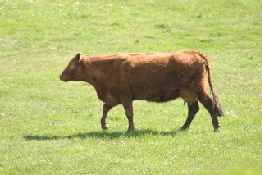
\includegraphics[width=4cm,keepaspectratio]{images/img.pdf}
        \end{center}
        \caption{Referenční obrázek}
    \endminipage
    \hfill
    \minipage{0.3\textwidth}
        \begin{center}
            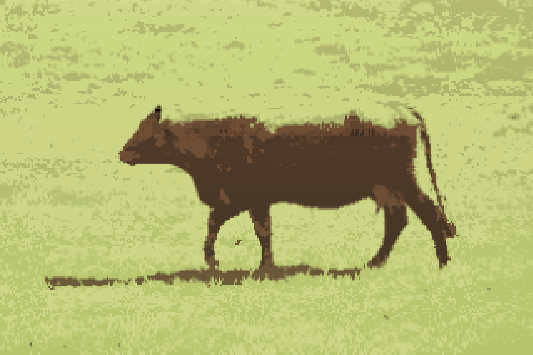
\includegraphics[width=4cm,keepaspectratio]{images/km.pdf}
        \end{center}
        \caption{K-means clustering}
    \endminipage
    \hfill
    \minipage{0.3\textwidth}
        \begin{center}
            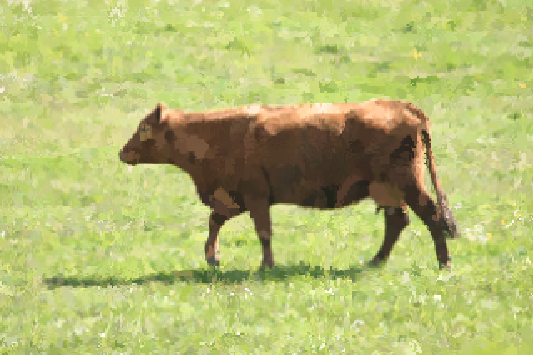
\includegraphics[width=4cm,keepaspectratio]{images/ms.pdf}
        \end{center}
        \caption{Mean-shift clustering}
    \endminipage
\end{figure}


%---------------------------------------------------------------------------
\section{Ovládání vytvořeného programu}
Výsledný program má podobu konzolové aplikace pracující dávkově. Program po volbé parametrů při spuštění (viz níže) provede samotný výpočet a na obrazovku zobrazí výsledek. Aplikace vypne standardním stiskem \texttt{Esc} nebo \texttt{Q}.

Spuštění programu s~parametry:
\begin{itemize}
  \item Zpracování metodou k-means 
    \begin{itemize}
      \item[] \texttt{./gmu km FILE}
    \end{itemize}
  \item Zpracování metodou mean-shift
    \begin{itemize}
      \item[] \texttt{./gmu ms FILE}
    \end{itemize}
\end{itemize}
kde \texttt{FILE} odpovídá vstupnímu obrázku, který bude segmentován.


%---------------------------------------------------------------------------
\section{Rozdělení práce v~týmu}
Práce byla rozdělena mezi členy týmu následovně:
\begin{itemize}
\item Martin Šimon - algoritmus mean-shift, experimenty s~OpenCL
\item Pavel Širůček - algoritmus k-means, optimalizace OpenCL
\end{itemize}

Práce v~týmu byla rozdělena rovnoměrně a to již na první společné konzultaci. Při tomto rozdělení jsme i zůstali. Části zde nezmíněné (dokumentace, návrh, apod.) byly výsledkem úzké spolupráce nás obou.

%---------------------------------------------------------------------------
\section{Co bylo nejpracnější}
Jako nejpracnější se ukázalo ladění samotných algoritmů, a to především kvůli netriviálnímu způsobu ladění paralelních systémů. Ke spokojenosti nepřispíval ani fakt rozdílných implementací OpenCL napříč různými platformami, což bylo problematické především u~starších strojů (soukromých). Samotná práce s~OpenCL a hledání vhodných parametrů paralelizace problém nezpůsobilo.

%---------------------------------------------------------------------------
\section{Zkušenosti získané řešením projektu}
Projekt nám přinesl praktické zkušenosti z~řešení problematiky obecných výpočtů na grafické kartě za pomoci OpenCL. Nedílnou součástí bylo hluboké pochopení segmentačních algoritmů k-means a mean-shift. Prohloubení znalostí C/C+++ provází snad každý projekt, kde jsou tyto technologie použity.

%---------------------------------------------------------------------------
\section{Autoevaluace}
\paragraph{Technický návrh (80\%):}
Projekt celý je postaven na programu z~2. cvičení předmětu GMU 2013, tudíž byl technický návrh zaměřen na reálné řešení problematiky paralelizace algoritmů. Algoritmy byly empiricky paralelizovány se snahou o~co nejvyšší výsledný výkon, což na jednu stranu nebyl nejlepší přístup, ale na druhou stranu přinesl žádoucí akceleraci.

\paragraph{Programování (75\%):}
Triviální znovupoužitelnost je ztížena neobjektivitou návrhu a práce s~OpenCL, na druhou stranu recyklace kernelů v~OpenCL je nasnadě. Program není plně odladěn, ostatně o~to nebyla ani přílišná snaha. Cílem bylo akcelerovat výpočty, což jsme také v~řešení vhodně demonstrovali.

\paragraph{Vzhled vytvořeného řešení (65\%):}
Aplikace je konzolová, krom zobrazení výsledku segmentace a průběžných výpisů na standardní vstup ani nic nevypisuje. Estetická kvalitě výsledků segmentace byla v~rámci řešení přiřazena nižší priorita, tudíž nebylo ani cílem, aby výsledky segmentace byly bezchybné.

\paragraph{Využití zdrojů (90\%):}
Celý projekt je založen na (recyklovaném) programu z~2. cvičení předmětu GMU 2013 a algoritmy jsou implementovány podle referenčních vzorců. V~celém projektu pak až na vyjímky nebylo třeba vytvářet nové postupy řešení a tak byly zdroje využity takřka stoprocentně.

\paragraph{Hospodaření s~časem (95\%):}
Práce na projektu začaly s~velkým předstihem, pracovalo se průběžně, výsledné řešení bylo hotovo několik dní před odevzdáním aniž bychom se dostali do časového tlaku.

\paragraph{Spolupráce v~týmu (95\%):}
Komunikace v~týmu probíhala pravidelně, došlo na několik osobních konzultací a velkou výhodou bylo, že každý člen týmu měl přehled o~postupu a problémech dalšího člena týmu. K~plné spokojenosti jsme používali verzovací systém, několik elektronických komunikačních kanálů a již zmíněné osobní konzultace.

\paragraph{Celkový dojem (80\%):}
Zadání jsme zvolili jako takové, které požaduje implementaci obecného výpočtu na grafické kartě tak, jak bylo OpenCL navrženo. Domníváme se, že jsme zadání dodrželi a úspěšně dosáhli požadované akcelerace. Projekt nám také dal očekávané praktické znalosti o~obecných výpočtech na grafické kartě.

%---------------------------------------------------------------------------
\section{Doporučení pro budoucí zadávání projektů}
Cílem bylo naučit se implementovat obecné výpošty na grafické kartě. Tento cíl byl dosažen, nicméně chvílemi nastávala situace, kdy implementace a dekompozice algoritmu (ne vzhledem k~paralelizaci) byla složitější než samotné využití paralelizačních mechanismů poskytovaných platformou OpenCL. Požadované algoritmy by měly být hloupé až naivní ve smyslu jednoduché implementace za cenu velkého vypočetního výkonu, aby nebylo těžké je implementovat a dosažené zrychlení bylo markantní.


\end{document}
% vim:set ft=tex expandtab enc=utf8:
